\documentclass{article}
\usepackage[utf8]{inputenc}
\usepackage[main=russian,english]{babel}
\usepackage{caption}
\usepackage{subcaption}
\usepackage{graphicx}
\usepackage{hyperref}

\title{Lab work $10_1$\\ HOPLS }

\author{Safiullin Robert} 
\date{}
\begin{document}
\maketitle

\addtocontents{toc}{\setcounter{tocdepth}{-10}}


\subsection*{Motivation}

The purpose of this work was to test the applicability of the higher-order partial least squares algorithm to actual microscopy problems

\subsection*{Problem statement}

Check the optimal method for working with for multiway data. The data are images from an atomic force microscope of the form $\mathbf{T}\in R^{\mathbf{X}\times \mathbf{Y}\times \mathbf{I}}$, where $\mathbf{X},\mathbf{Y}$ are the coordinates of the surface under study for a given resolution, and \mathbf{I} are the values of some function of the shift of the amplitude-frequency and phase-frequency characteristics of the oscillations of the microscope probe.
\subsection*{Problem solution}
\textbf{HOPLS}
\begin{left}

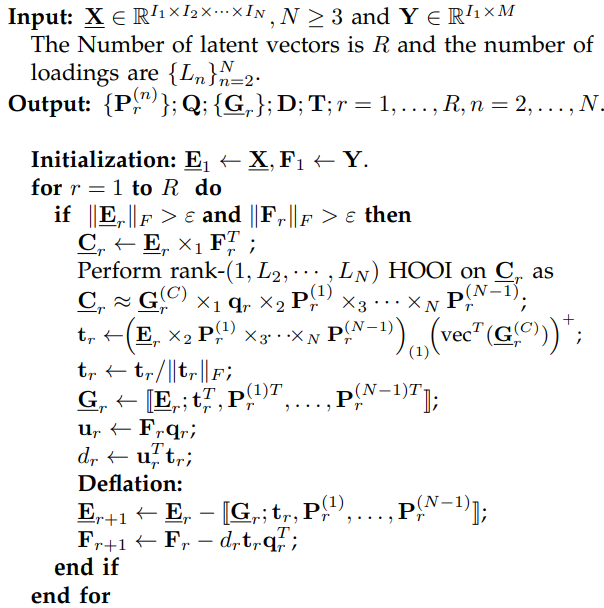
\includegraphics[scale = 0.45]{im1.png}
\end{left}


\subsection*{Experiment}
\begin{center}
    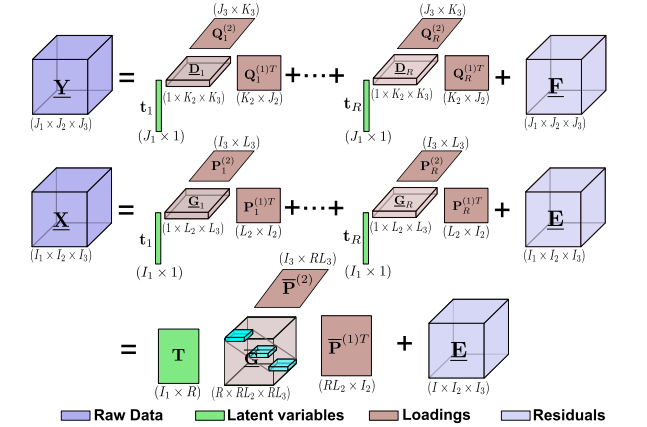
\includegraphics[scale = 0.5]{im2.png}
\end{center}
Let's consider how the residual tensor of the $E_r$  changes depending on the number of their original hidden vectors removed. \\

We also visualize the distribution of data in the space of these vectors.
\newpage


\begin{figure}[!htb]
\minipage{0.23\textwidth}
  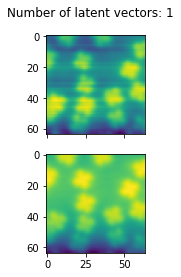
\includegraphics[width=\linewidth]{11.png}
\endminipage\hfill
\minipage{0.23\textwidth}
  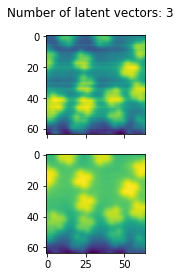
\includegraphics[width=\linewidth]{13.png}
\endminipage\hfill
\minipage{0.23\textwidth}%
  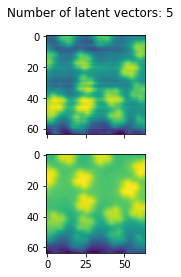
\includegraphics[width=\linewidth]{15.png}
\endminipage
\minipage{0.23\textwidth}%
  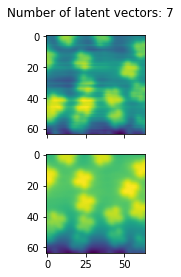
\includegraphics[width=\linewidth]{17.png}
\endminipage
\caption{Dependence of $\mathbf{}{E^r_1} (R)$}
\end{figure}



\begin{figure}[!htb]
\minipage{0.23\textwidth}
  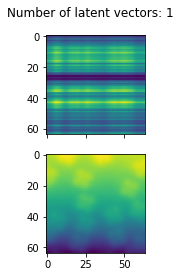
\includegraphics[width=\linewidth]{21.png}
\endminipage\hfill
\minipage{0.23\textwidth}
  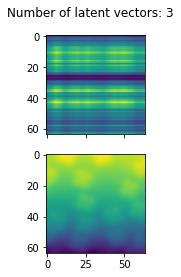
\includegraphics[width=\linewidth]{23.png}
\endminipage\hfill
\minipage{0.23\textwidth}%
  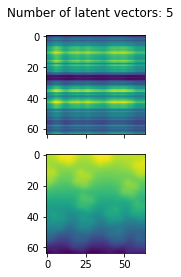
\includegraphics[width=\linewidth]{25.png}
\endminipage
\minipage{0.23\textwidth}%
  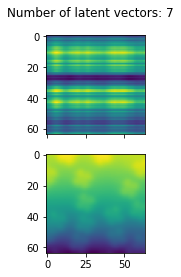
\includegraphics[width=\linewidth]{27.png}
\endminipage
\caption{Dependence of $\mathbf{}{E^r_2} (R)$}
\end{figure}

\newpage


\begin{figure}[!htb]
\minipage{0.45\textwidth}
  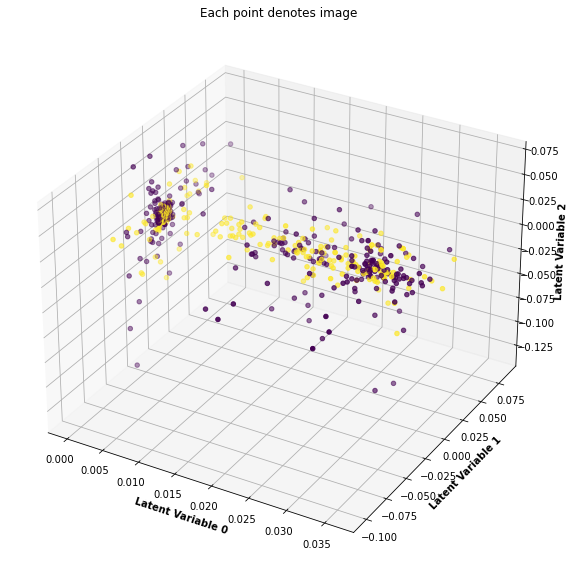
\includegraphics[width=\linewidth]{1_.png}
\endminipage\hfill
\minipage{0.45\textwidth}%
  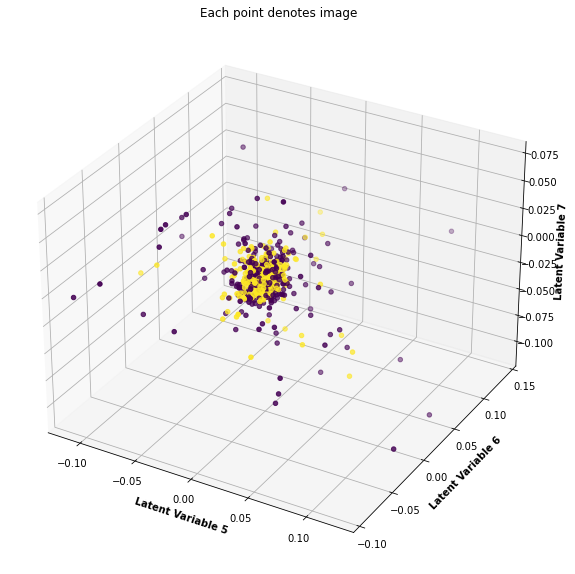
\includegraphics[width=\linewidth]{1__.png}
\endminipage
\caption{Distibution of data in $ R^{LV_i \times LV_j \times LV_k}$}
\end{figure}


\begin{figure}[!htb]
\minipage{0.45\textwidth}
  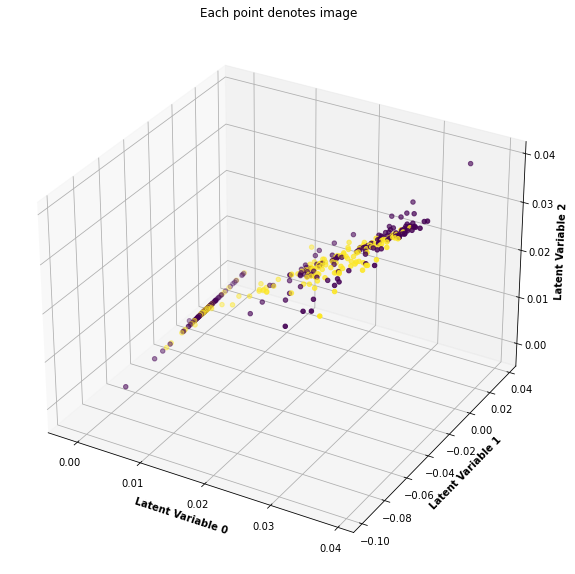
\includegraphics[width=\linewidth]{2_.png}
\endminipage\hfill
\minipage{0.45\textwidth}%
  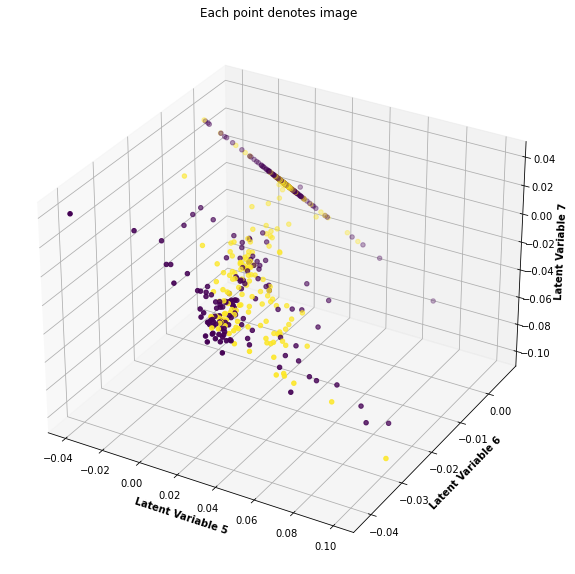
\includegraphics[width=\linewidth]{2__.png}
\endminipage
\caption{Distibution of data in  $ R^{LV_i \times LV_j \times LV_k}$}
\end{figure}

\subsection*{Approximation results}
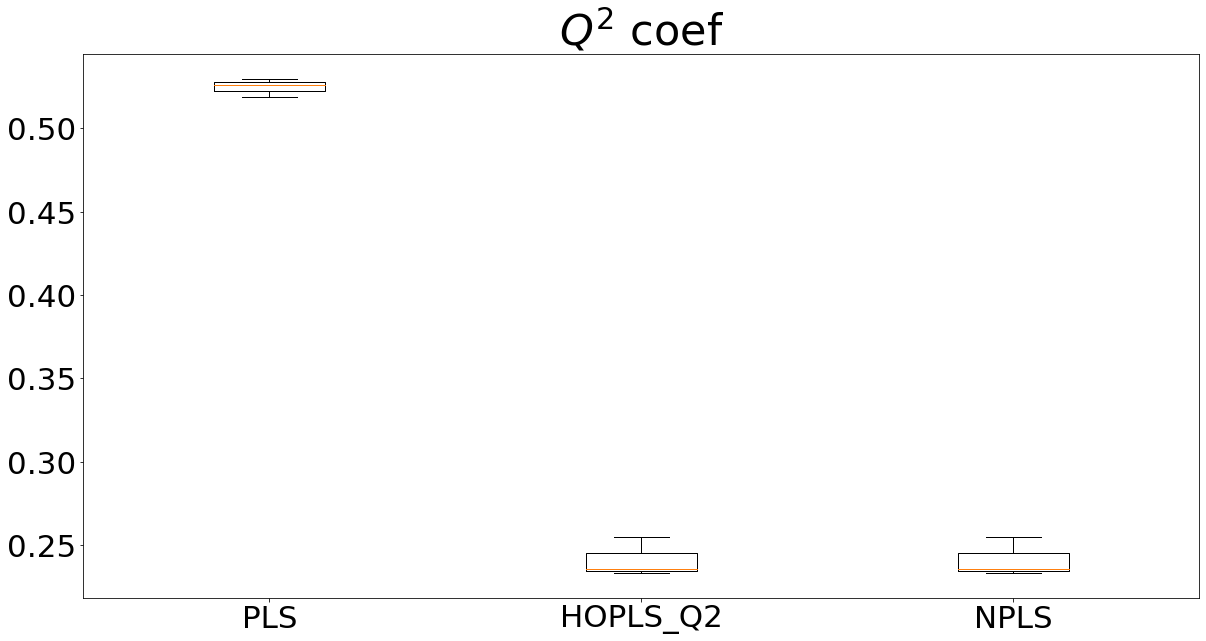
\includegraphics[scale = 0.25]{323.png}\\

\begin{center}
    

$Q^2 = 1- \left\lVert \mathbf{Y} - \widetilde{\mathbf{Y}} \right\lVert^2_F /\left\lVert \mathbf{Y} \right\lVert^2_F  $
\end{center}
\newpage
\subsection*{Supplementary}
\href{https://arxiv.org/pdf/1207.1230.pdf}{HOPLS} \\
\href{https://github.com/roberts2510/MMoF}{Github}\\
\href{https://www.nature.com/articles/s42005-020-0317-3}{Data}

\end{document}